% This is the template used for the GIH thesis. It is based on 
% Reed College LaTeX thesis template. Most of the work (Reed template)
% for the document class was done by Sam Noble (SN), as well as this
% template. Later comments etc. by Ben Salzberg (BTS). Additional
% restructuring and APA support by Jess Youngberg (JY).
%
% See http://web.reed.edu/cis/help/latex.html for help. There are a
% great bunch of help pages there, with notes on
% getting started, bibtex, etc. Go there and read it if you're not
% already familiar with LaTeX.
%
% Any line that starts with a percent symbol is a comment.
% They won't show up in the document, and are useful for notes
% to yourself and explaining commands.
% Commenting also removes a line from the document;
% very handy for troubleshooting problems. -BTS

% The template was updated by Daniel Hammarström to fit GIH
% requirements. Additional code was borrowed from the 
% Stockholm University (Andreas Solders 2011) template.

% The template was forked from the thesisdown package (CII updates)

%%
%% Preamble
%%
% \documentclass{<something>} must begin each LaTeX document
\documentclass[twoside,10pt]{gihclass} %Default style using S5 paper
% Packages are extensions to the basic LaTeX functions. Whatever you
% want to typeset, there is probably a package out there for it.
% Chemistry (chemtex), screenplays, you name it.
% Check out CTAN to see: http://www.ctan.org/
%%
\usepackage{graphicx,latexsym}
\usepackage{amsmath}
\usepackage{amssymb,amsthm}
\usepackage{longtable,booktabs,setspace}
\usepackage{chemarr} %% Useful for one reaction arrow, useless if you're not a chem major
\usepackage[hyphens]{url}
% Added by CII
\usepackage{hyperref,xcolor}
\hypersetup{
    colorlinks = false,
    pdfborder={0 0 0}
}
\usepackage{lmodern}
\usepackage{float}
\floatplacement{figure}{H}
% End of CII addition
\usepackage{rotating}

% Next line commented out by CII
%%% \usepackage{natbib}
% Comment out the natbib line above and uncomment the following two lines to use the new
% biblatex-chicago style, for Chicago A. Also make some changes at the end where the
% bibliography is included.
%\usepackage{biblatex-chicago}
%\bibliography{thesis}


% Added by CII (Thanks, Hadley!)
% Use ref for internal links
\renewcommand{\hyperref}[2][???]{\autoref{#1}}
\def\chapterautorefname{Chapter}
\def\sectionautorefname{Section}
\def\subsectionautorefname{Subsection}
% End of CII addition

% Added by CII
\usepackage{caption}
\captionsetup{width=5in}
% End of CII addition


% \usepackage{times} % other fonts are available like times, bookman, charter, palatino


% Syntax highlighting #22

% To pass between YAML and LaTeX the dollar signs are added by CII

% New variables 2019-02-06 GIH copyright info 
\isbn{Provided by the library} 
\place{Stockholm}
\printeby{Printer service, Stockholm, 2019}
\coverinfo{}
\year{2019}



\title{Determinants of intra-individual variation in adaptability to resistance training of different volumes with special reference to skeletal muscle phenotypes}
\author{Daniel Hammarström}
% The month and year that you submit your FINAL draft TO THE LIBRARY (May or December)
\date{May 20xx}


%If you have two advisors for some reason, you can use the following
% Uncommented out by CII
\sernr{999}
% End of CII addition
%%% Remember to use the correct department!

% if you're writing a thesis in an interdisciplinary major,
% uncomment the line below and change the text as appropriate.
% check the Senior Handbook if unsure.
%\thedivisionof{The Established Interdisciplinary Committee for}
% if you want the approval page to say "Approved for the Committee",
% uncomment the next line
%\approvedforthe{Committee}

% Added by CII
%%% Copied from knitr
%% maxwidth is the original width if it's less than linewidth
%% otherwise use linewidth (to make sure the graphics do not exceed the margin)
\makeatletter
\def\maxwidth{ %
  \ifdim\Gin@nat@width>\linewidth
    \linewidth
  \else
    \Gin@nat@width
  \fi
}
\makeatother

\renewcommand{\contentsname}{Table of Contents}
% End of CII addition

\setlength{\parskip}{0pt}

% Added by CII

\providecommand{\tightlist}{%
  \setlength{\itemsep}{0pt}\setlength{\parskip}{0pt}}




\Dedication{
You can have a dedication here if you wish.
}

\Preface{

}

\Abstract{
The preface pretty much says it all.

\par

Second paragraph of abstract starts here.
}

\Listofpapers{
\begin{enumerate}
\def\labelenumi{\Roman{enumi}.}
\item
  \textbf{Hammarström D}, Øfsteng S, Koll L, Hanestadhaugen M, Hollan I, Apró W, Blomstrand E, Rønnestad B, Ellefsen S Benefits of higher resistance-training volume are related to ribosome biogenesis. The \emph{Journal of physiology}. 2020 Feb;598(3):543-565. doi: 10.1113/JP278455.
\item
  Khan Y, \textbf{Hammarström D}, Rønnestad B, Ellefsen S, Ahmad R Increased biological relevance of transcriptome analyses in human skeletal muscle using a model-specific pipeline. \emph{BMC Bioinformatics}. 2020 Nov 30;21(1):548. doi: 10.1186/s12859-020-03866-y
\item
  \textbf{Hammarström D}, Øfsteng S, Jacobsen N, Flobergseter K, Rønnestad B, Ellefsen S Ribosome accumulation during early phase resistance training. \emph{Manuscript}
\end{enumerate}
}


	\usepackage{lettrine} \usepackage{booktabs} \usepackage{longtable} \usepackage{array} \usepackage{multirow} \usepackage{wrapfig} \usepackage{float} \usepackage{colortbl} \usepackage{pdflscape} \usepackage{tabu} \usepackage{threeparttable} \usepackage{threeparttablex} \usepackage[normalem]{ulem} \usepackage{makecell} \usepackage{siunitx}
	\usepackage{booktabs}
 \usepackage{longtable}
 \usepackage{array}
 \usepackage{multirow}
 \usepackage{wrapfig}
 \usepackage{float}
 \usepackage{colortbl}
 \usepackage{pdflscape}
 \usepackage{tabu}
 \usepackage{threeparttable}
 \usepackage{threeparttablex}
 \usepackage[normalem]{ulem}
 \usepackage{makecell}
% End of CII addition
%%
%% End Preamble
%%
%


% Added updated related to csl update in Pandoc
\newlength{\cslhangindent}
\setlength{\cslhangindent}{1.5em}
\newlength{\csllabelwidth}
\setlength{\csllabelwidth}{3em}
\newenvironment{CSLReferences}[3] % #1 hanging-ident, #2 entry spacing
 {% don't indent paragraphs
  \setlength{\parindent}{0pt}
  % turn on hanging indent if param 1 is 1
  \ifodd #1 \everypar{\setlength{\hangindent}{\cslhangindent}}\ignorespaces\fi
  % set entry spacing
  \ifnum #2 > 0
  \setlength{\parskip}{#2\baselineskip}
  \fi
 }%
 {}
\usepackage{calc} % for \widthof, \maxof
\newcommand{\CSLBlock}[1]{#1\hfill\break}
\newcommand{\CSLLeftMargin}[1]{\parbox[t]{\maxof{\widthof{#1}}{\csllabelwidth}}{#1}}
\newcommand{\CSLRightInline}[1]{\parbox[t]{\linewidth}{#1}}
\newcommand{\CSLIndent}[1]{\hspace{\cslhangindent}#1}


\begin{document}




% Everything below added by CII


\frontmatter % this stuff will be roman-numbered
% \pagestyle{empty} % this removes page numbers from the frontmatter
  \maketitle
  \begin{dedication}
  \topskip0pt
\vspace*{\fill}
 You can have a dedication here if you wish.
\vspace*{\fill}
  \end{dedication}
\begin{defence}
    THESIS FOR DOCTORAL DEGREE (Ph.D.)\\
    ~\\
    ~\\
    \textbf{The title of your thesis}\\
    ~\\
    by\\
    \textbf{Your name}\\
    ~\\
    ~\\
    Thesis for Philosophy of Doctoral Degree in Sport Sciences, at The Swedish School of Sport and Health Sciences (GIH), which, according to the decision of the dean, will be publicly defended on \emph{DATE}. The thesis defense will be held at the auditorium at The Swedish School of Sport and Health Sciences (GIH), Stockholm.\\
    ~\\
    ~\\
    \textbf{Opponent}\\
    Profesor \ldots.\\
    ~\\
    \textbf{Principal supervisor}\\
    Profesor\ldots{}\\
    ~\\
    \textbf{Co-supervisor(s)}\\
    -Professor\ldots{}\\
    -Professor\ldots{}\\
    -Professor\ldots{}\\
    ~\\
    \textbf{Examination board}\\
    -Associate professor\ldots{}\\
    -Professor \ldots{}\\
    -Professor \ldots{}
  \end{defence}

  \begin{abstract}
    The preface pretty much says it all.

    \par

    Second paragraph of abstract starts here.
  \end{abstract}
  \begin{listofpapers}
    \begin{enumerate}
    \def\labelenumi{\Roman{enumi}.}
    \item
      \textbf{Hammarström D}, Øfsteng S, Koll L, Hanestadhaugen M, Hollan I, Apró W, Blomstrand E, Rønnestad B, Ellefsen S Benefits of higher resistance-training volume are related to ribosome biogenesis. The \emph{Journal of physiology}. 2020 Feb;598(3):543-565. doi: 10.1113/JP278455.
    \item
      Khan Y, \textbf{Hammarström D}, Rønnestad B, Ellefsen S, Ahmad R Increased biological relevance of transcriptome analyses in human skeletal muscle using a model-specific pipeline. \emph{BMC Bioinformatics}. 2020 Nov 30;21(1):548. doi: 10.1186/s12859-020-03866-y
    \item
      \textbf{Hammarström D}, Øfsteng S, Jacobsen N, Flobergseter K, Rønnestad B, Ellefsen S Ribosome accumulation during early phase resistance training. \emph{Manuscript}
    \end{enumerate}
  \end{listofpapers}

  \hypersetup{linkcolor=black}
  \setcounter{tocdepth}{2}
  \tableofcontents

  \listoftables

  \listoffigures




\mainmatter % here the regular arabic numbering starts
\pagestyle{fancyplain} % turns page numbering back on

\setcounter{DefaultLines}{3}

\hypertarget{introduction}{%
\chapter{Introduction}\label{introduction}}

\lettrine{S}keletal muscle health is essential for physical independence. In a lifespan perspective, measures of muscle mass and/or strength are inversely associated with mortality
(1, 2, 3, 4, 5, 6)
and disability
(7).
Besides adverse associations between of low muscle mass and strength and clinical conditions, muscle weakness also accounts for increased health care costs in patient populations
(8, 9).
The intercept between muscle mass, muscle function and health status is interrelated with variables such as age and primary illness or injury
(10).
This highlights that interventions designed to increase muscle mass and strength are likely to prevent adverse health outcomes across the lifespan. A higher level of muscle mass and functional capacity would counteract the effects of muscle loss due to illness, age or inactivity.

Although a large degree of the observed variations in lean mass and strength are attributed to genetic components
(11, 12),
environmental factors also contribute, leaving a window of opportunity to increase muscle mass and functional capacity. Among factors affecting muscle mass and functioning are nutrition and pharmacological agents. However, physical activity and specifically systematic resistance training of sufficient volume, intensity and frequency provides a stimulus that promote morphological and functional changes to the human neuromuscular system without adverse side-effects. Irrespective of age, resistance training generally leads to increased muscle mass and strength
(13, 14)
and is considered safe when performed in a well organized manner
(14, 15).

Resistance training can be modulated indefinitely through combined variations of training variables such as frequency, intensity and volume
(16, 17).
Well designed training prescriptions should incorporate information about the current state and goals of the trainee to maximize the potential outcome of the training program
(16, 18, 17).
Training volume has received particular attention in the scientific community for many reasons. Evidence suggests that exercise volume affects selected molecular determinants of muscle hypertrophy in a dose-dependent manner
(19, 20, 21).
Such effects are believed to facilitate long-term training effects as training programs with higher volume generally result in higher gains in muscle mass and strength with little evidence of differences between age groups or participants with different training backgrounds
(22, 23, 24). \\
A consequence of a more extensive training program is the increased time required to complete such a program. As time constraints has been reported as a limiting factor for engaging in physical activity
(25)
some merit can be given to arguments against guidlines suggesting higher volume in resistance training prescription
(26, 18).
From an individual perspective, training prescription that balances time-requirement with efficacy presumably increases the likelihood of participation in physical activity (25).
From a more general perspective, increased knowledge about mechanisms governing responses to physical training could improve training prescription also for individuals and populations that experience attenuated benefit of resistance training
(27).
The overreaching goal of the present thesis is to contribute to understanding individualized training loads. To this end, training volume was used to study the effects of variable training stimulus in within-participant models of exercise-training.

\hypertarget{background}{%
\chapter{Background}\label{background}}

\hypertarget{progressive-resistance-exercise-prescription-a-brief-historical-note-and-current-challenges}{%
\section{Progressive resistance exercise prescription, a brief historical note and current challenges}\label{progressive-resistance-exercise-prescription-a-brief-historical-note-and-current-challenges}}

Recommendations of systematic physical exercise with the purpose to improve health or physical performance has long been part of human culture, evident from records dating back to ancient Chinese, Indian and Greek civilizations
(28).
Today's exercise-training prescription still bears traces of ideas from these eras, further developed during the renaissance and formalized in systems like German Turnen and Ling gymnastics during the nineteenth century
(29).
Especially Ling gymnastics was important for the development of modern exercise prescription as it was scientifically oriented, based on the then current physiological and medical understanding (29).
Development of a medical gymnastics during the nineteenth century in turn is referenced in twentieth century texts on therapeutic exercise prescription
(30).

With the introduction of ``heavy resistance exercises'' for the development of muscle strength and mass after injury, DeLorme outlined a system on which modern resistance-training exercise prescription is based (31).
DeLorme published his system short after the Second World War (31)
during which he, as a newly graduated physician, had been working with war injury rehabilitation
(32).
Inspired by practitioners of weight training (32),
DeLorme specifically emphasized high-resistance, low-repetition exercise where progression was achieved with increased resistance (31) as opposed to previous recommendations of endurance-like exercise where progression was achieved through increased number of repetitions
(30).
DeLorme originally used the term ``heavy resistance exercises'' in contrasts to low-resistance exercises (31), but as this could be perceived as exercises performed only with heavy weights, the system was renamed \emph{progressive resistance exercise} to better reflect the method
(33).
Indeed, central to the system was the concept of repetition maximum as a way of prescribing an individual load and monitoring progress (31).
DeLorme originally prescribed sessions of up to 100 repetitions performed in sets of 10 repetitions (31) but later revised this recommendation to three sets of 10 repetitions performed with increasing intensities
(33).

Scientific inquiries into prescription of resistance training from the first part of the twentieth century concerned its therapeutic use
(e.g. 31, 34)
but also came to be introduced as a means of improving strength and physical performance in healthy populations
(e.g. 35, 36, 37).

Scientific contributions soon moved from questions regarding the effectiveness of resistance training \emph{per se} to comparing outcomes from different modes of resistance training
(38, 39, 40, 41, 42, 43).
A vocabulary for progressive resistance exercise-training developed through these investigations and parallel practice,
the introduction of repetition maximum by DeLorme being one example. These concepts established as modern definitions of exercise variables enabling precise prescription of training loads for a variety of populations and training goals
(17).

Although this development started after the Second World War, resistance training was not part of general exercise guidelines until much later.
The American College of Sports Medicine (ACSM) position statement on exercise for healthy individuals from 1978 (45)
primarily concerned physical fitness in terms of cardio-respiratory fitness.
Since the updated 1990 ACSM statement, resistance training is recommended to be included as part of a sensible, general training program (46).
The introduction of resistance-training as part of the ACSM recommendation also marks the start of specific recommendations on resistance training being part of other consensus statements
(47, Ch. 2).
Consequently, informed by epidemiological data, the most recent general guidelines for physical activity do include resistance training (48).

It could be argued that the above account reflects the fact that common understandings of \emph{why} and \emph{how to} exercise are influenced by societal norms and historic events such as the search of national identity in the nineteenth century or war injuries in the twentieth century
(29,32).
A current influence on exercise science is the development of cheap techniques to collect large amount of biological data, something that could be exemplified with the continuously decreasing cost of a sequenced human genome
(49).
The development of such molecular techniques has enabled efforts to describe mechanisms by which exercise training induce favorable adaptations. The newly established Molecular Transducers of Physical Activity Consortium is an example of a large scale effort, explicitly initiated to develop personalized exercise recommendations and identify molecular targets through which effects of exercised may be mimicked (50).
Advances in bio-medical technologies are enablers of this enterprise and the quest to \emph{individualize} exercise based on molecular diagnostics can be seen as a motivation for modern exercise science
(50, 51).

A challenge facing this enterprise is to accurately describe etiologies of response heterogeneity associated with physical training. A wide variation of individual responses are commonly observed after standardized progressive resistance training programs where measures of muscle strength-changes varies from -32 to +250\% and muscle size-changes varies from negative to (-11\%) to impressively large (+59\%)
(52, 13).
By relating such variations to individuals genome (DNA)
(53),
and messenger RNA (mRNA) profiles
(54, 55)
we are beginning to gain knowledge about the genetic influence on training responses.

The rise of data intensive techniques also highlights the complexity associated with ``molecular exercise prescription.'' In simplistic terms, genetic information is transferred from DNA to RNA through transcription and from RNA to protein through translation. This flow of information, known as the central dogma of molecular biology
(56)
indicates a deterministic role of DNA in controlling the characteristics of an organism. It is however apparent that the transcription of specific genes are under tight control of several mechanisms including a group of non-genetic modifications to the DNA organization of each cell known as epigenetic modifications
(57, 58).
Such control determines gene expression in response to progressive resistance training with modifications persisting after a period of de-training
(59, 60).
Regulation of gene expression is thus related to modifiable variables such as exercise and diet
(57, 58, 61, 62)
linking environmental factors to the complexity of gene expression.

In the study of response heterogeneity, a common strategy has been to dichotomize responses into ``responders'' and ``non-responders'' to exercise training. From e.g.~a public health perspective this is probably fruitful when \emph{non-response} is defined as the absence of meaningful health-related adaptations, or even adverse effects in response to a given training regime
(51, \textbf{RN2698?}).
Such effects would have large implications regarding exercise prescription on the population scale
(63).
The full potential of exercise prescription based on molecular diagnostics in reducing non- or adverse-response to a given training regime possibly lies in the future
(\textbf{RN2698?}, 27).
In such a scenario, a key aspect of successful exercise diagnostics would be to map the relationship between exercise variables (i.e.~modality, intensity, volume etc.) and exercise response for different phenotypes.
It seems for example that an individual classified as non-responsive to a specific exercise modality (e.g.~endurance training) may be classified as a responder to another (e.g.~resistance training)
(64).
Even changing training variables within a specific modality have been shown to convert non-responders to responders as endurance training volume was increased
(\textbf{RN2699?}).

By manipulating exercise variables in within-participant models we could potentially further our understanding of whom would benefit from a specific manipulation in addition to exploring possible mechanism behind such variability.

\hypertarget{adaptations-to-resistance-training}{%
\section{Adaptations to resistance training}\label{adaptations-to-resistance-training}}

\hypertarget{muscle-hypertrophy-and-strength}{%
\subsection{Muscle hypertrophy and strength}\label{muscle-hypertrophy-and-strength}}

A well characterized response to systematic resistance training in humans is muscle growth. In healthy, untrained individuals regardless of age, resistance training can be expected to result in increases of \textasciitilde{} 5-20\% when training is conducted over two weeks to 6 months
(13, 65, 52).
Responses can be expected to be more pronounced in upper- compared to the lower-body muscles
(65)

(66)

(67)

(68)

(69)

\hypertarget{muscle-fiber-type-transitions}{%
\subsection{Muscle fiber-type transitions}\label{muscle-fiber-type-transitions}}

\hypertarget{mitochondrial-function}{%
\subsection{Mitochondrial function}\label{mitochondrial-function}}

Increased mitochondrial respiration after 12 weeks of RT in young men (70)

Fiber type distributions do not predict muscle mitochondrial density in endurance trained individuals (71)

\url{PMID:158694} Reduced mitochondrial density per fiber area in reponse to RT

\hypertarget{effects-of-exercise-prescription-on-muscle-mass-and-strength}{%
\section{Effects of exercise prescription on muscle mass and strength}\label{effects-of-exercise-prescription-on-muscle-mass-and-strength}}

Precise exercise-training\footnote{Exercise is herein defined as an acute bout of physical activity designed to affect physical characteristics such as strength, speed or endurance. Training is defined as the systematic process of combining multiple exercise-sessions performed in sequence over time. Resistance-exercise is defined as an acute strength-promoting program requiring the neuromuscular system to exert force against resistance. Resistance training is defined as a long-term process of multiple resistance exercise-sessions performed over a defined period of time.}
prescription gives information on exercises, their sequential order, intensity and volume, rest periods between efforts or sessions and the frequency at which exercise sessions are to be performed
(23).
By manipulating these variables, resistance training programs can be tailored to better fit goals and starting points of any individual.
The relative importance of exercise-training variables for training outcomes has been examined in numerous studies including (but not limited to) the overall organization of exercise sessions,
(72, 73)
training frequency
(74),
and intensity
(75).
It could be argued that training volume is of particular importance for muscle growth as when this variable is held constant, manipulation of other variables has little or no effect hypertrophy
(76, 75).
For development of strength, factors such as intensity and within session organization of exercises is of importance
(77, 78),
however, when other factors are held constant, increased training volume generally leads to increased strength
(77,79, 22),
similarly to effects of training volume on muscle growth
(23,24).

\hypertarget{effects-of-resistance-exercise-volume-on-muscle-strength-and-mass}{%
\subsection{Effects of resistance exercise volume on muscle strength and mass}\label{effects-of-resistance-exercise-volume-on-muscle-strength-and-mass}}

Exercise volume can be prescribed as the within session number of sets performed per muscle group. This unit is practical as it comparable between individuals and muscle groups (80).
Berger conducted an early study concerning effects of resistance exercise volume with the goal to determine what method most efficiently produced strength gains (in healthy young males) (81). Berger compared one, two and three sets performed with two, six or ten repetition maximum (RM) in the bench press, three times per week, over twelve weeks. As the combined effect of three sets per session was superior regardless of the number of repetitions performed Berger concluded in favor of three sets. This conclusion was later challenged on the basis of data interpretation
(26, 18).
Reveiwing the study by Berger and others, Carpinelli and Otto arrived to the conclusion that there was ``insufficient evidence to support the prevalent belief that a greater volume of exercise (through multiple sets) will elicit superior muscular strength or hypertrophy'' (26). This stand has since been repeatedly put forward as a criticism of higher volume training programs
(82,83) and sparked considerable scientific activity. The main argument against the recommendation of additional volume in strength training programs has been the lack of statistically significant results in single studies (18,82).
Indeed, individual studies do not generally agree on dose-dependent effects of training volume on muscle mass and strength gains
(84, 85, 86, 87, 88, 89, 40, 90, 91, 92, 93, 94),
including studies performed within participants, where different training volumes are allocated to either extremity
(95, 96).
For example, differences in strength are between volume conditions are found in older individuals
(84, 85, 40)
but not confirmed in another study
(88){]}.
Studies shows that more volume does not lead to increased muscle gains in young individuals
(92, 90, 86)
a conclusion challenged by others
(94, 87).

As previously noted, combining the above results and additional studies, meta-analyses concluded that training volume dose-dependency exists for the development of muscle mass and strength
{[}(77);
(79);
(22);
(23,24).
As a second argument against additional volume in resistance training recommendation has been the cost/benefit relationship of adding training volume without meaningful or substantial additional gains
(18, 82),
a subsequent question is, whom would benefit from greater volumes and whom would not?
Schoenfeld \emph{et al.} combined data from published studies to explore if participant characteristics of the above mentioned studies interacted with training volume in explaining study outcomes. Neither sex, muscle groups nor age interacted with volume prescription indicating that no such factor would be able refine training prescription guidelines
(24).
As the number of studies used to synthesis the meta-analysis was relatively low (\emph{n} = 15) and the studies were heterogeneous in terms of e.g.~outcome measurements, it may have lacked in power to detect any meaningful interactions. Additionally, included studies may not have been reporting relevant characteristics for such analysis.

Collectively, the available evidence suggest that there is overlap between training outcomes in studies were different volume has been utilized.
The overlap cannot, with available data, be explained by general population characteristics such as age or sex.
Studying the effect of different training volumes within participants could potentially help to define determinants of training outcomes in response to different volume conditions.
Two within-participant studies have investigated the effects of training volume on strength and hypertrophy outcomes.
Sooneste \emph{et al.} compared strength outcomes in response to three- and one-set elbow flexor training for 12 weeks in young males using a whitin-participant protocol (arms allocated to either volume condition).
The results showed general benefit of three- over one-set training for muscle hypertrophy and tended to do so also for strength gains (96).
No attempts were made to relate baseline characteristics to the magnitude of differences between volume conditions, presumably due to the small sample size (\emph{n} = 8).
Mitchell \emph{et al.} compared muscle hypertrophy and strength gains in response to three- and one-set of knee-extension exercise performed three times per week for ten weeks.
The study contained an additional training condition (low intensity, 30\% of 1RM performed with three sets) with participants legs assigned to either of the three conditions in a random fashion.
No significant differences were reported between volume conditions for muscle mass or strength gains (95).
However, the analyses were performed without taking the correlation between individuals into account due to the mixed design (95).
No attempts were made to relate any measured characteristic to differences in responses.

\hypertarget{molecular-determinants-of-training-induced-muscle-hypertrophy}{%
\section{Molecular determinants of training-induced muscle hypertrophy}\label{molecular-determinants-of-training-induced-muscle-hypertrophy}}

Muscle mass change as a consequence of muscle protein synthesis and breakdown. When a net positive balance is achieved the muscle increase in mass. Resistance exercise leads ta acute blunting of muscle protein synthesis followed by an increase over resting levels in the post exercise period
.
.

\hypertarget{ribosomal-biogenesis}{%
\subsection{Ribosomal biogenesis}\label{ribosomal-biogenesis}}

(97)
(98)

(99)

\hypertarget{transcriptional-regulation-of-muscle-mass}{%
\subsection{Transcriptional regulation of muscle mass}\label{transcriptional-regulation-of-muscle-mass}}

(100)

(101)

.

.

\hypertarget{aims}{%
\chapter{Aims}\label{aims}}

The primary aim of this thesis was to relate the adaptive response to resistance training with low- and moderate-volume to skeletal-muscle characteristics in previously untrained individuals. The key question was whether manipulation of exercise-volume will have diverse effects in different individuals related to muscular intrinsic characteristics. A further aim was to characterize exercise-volume dependence in muscle molecular characteristics and determine a time course profile of markers of ribosomal biogenesis in response to resistance training. Based on these aims, the objectives of the present thesis were;
\begin{itemize}
\tightlist
\item
  to relate skeletal muscle and systemic characteristics to benefit of moderate- compared to low-volume resistance training;
\item
  To determine volume-dependence in molecular networks related to muscle growth and remodeling in response to resistance training
\item
  To determine a time course of markers related to ribosome biogenesis in the early phase of resistance training.
\end{itemize}
\hypertarget{methods}{%
\chapter{Methods}\label{methods}}

\hypertarget{study-participants-protocols-and-training-interventions}{%
\section{Study participants, protocols and training interventions}\label{study-participants-protocols-and-training-interventions}}

Study I was designed to examine effects of low- and moderate-volume on
responses to acute exercise and long-term training within participants.
Forty-one healthy individuals were recruited and 34 of these completed
at least 85\% of the prescribed sessions and were thus included in
subsequent data analyses. Reasons for not completing the trial included
injury not related to the study (\emph{n =} 1), pain or discomfort during
exercises (\emph{n =} 5) and non-adherence to the study protocol. There were
no differences in characteristics between participants included in or
excluded from data analysis in Study I.

Study II was designed to study the effects of resistance training \emph{per
se}, and effects of variable volume on selected markers related to
ribosome biogenesis. Participants were therefore recruited to a training
group (\emph{n =} 11) and a non-training control group (\emph{n =} 8). Eligible
for participation in both studies were young (Study I age 18-40; Study
II 18-35), non-smoking men and women. Exclusion criteria included a
training history of more than one weekly session during the last 12
(Study I) or six (Study II) months leading up to the study. Participants
were also screened for intolerance to local anesthetic, current or
previous injuries affecting their ability to perform resistance
training, self-reported symptoms or history of disease, intake of
medication or supplements with known effects on adaptations to training.
Participant characteristics for both studies are shown in Table
\ref{tab:characteristics-table}.
\begin{table}

\caption{\label{tab:characteristics-table}Participant characteristics}
\centering
\fontsize{7}{9}\selectfont
\begin{tabular}[t]{llllllll}
\toprule
  &   & Sex & Age (years) & Stature
(cm) & Mass (kg) & Fat mass (\%) & Lean mass (\%)\\
\midrule
 &  & Female & 22.0 (1.3) & 168 (7) & 64.4 (10.4) & 34.1 (5.6) & 64.3 (6.2)\\
\cmidrule{3-8}
 & \multirow{-2}{*}{\raggedright\arraybackslash Included} & Male & 23.6 (4.1) & 183 (6) & 75.8 (10.7) & 20.4 (6.0) & 79.3 (5.0)\\
\cmidrule{2-8}
 &  & Female & 22.9 (1.6) & 166 (8) & 64.6 (9.7) & 28.8 (8.7) & 68.6 (9.1)\\
\cmidrule{3-8}
\multirow{-4}{*}{\raggedright\arraybackslash Study I} & \multirow{-2}{*}{\raggedright\arraybackslash Excluded} & Male & 24.3 (1.5) & 189 (5) & 88.2 (22.4) & 24.3 (15.3) & 76.8 (12.7)\\
\cmidrule{1-8}
 &  & Female & 23.4 (2.9) & 168 (8) & 64.0 (9.2) & 30.8 (7.1) & 65.5 (6.8)\\
\cmidrule{3-8}
 & \multirow{-2}{*}{\raggedright\arraybackslash Training} & Male & 25.7 (5.8) & 177 (3) & 77.5 (8.0) & 25.3 (3.9) & 71.3 (2.4)\\
\cmidrule{2-8}
 &  & Female & 24.1 (3.5) & 166 (4) & 63.8 (0.6) & 30.5 (6.4) & 66.3 (5.2)\\
\cmidrule{3-8}
\multirow{-4}{*}{\raggedright\arraybackslash Study II} & \multirow{-2}{*}{\raggedright\arraybackslash Control} & Male & 25.5 (5.5) & 182 (5) & 76.5 (7.7) & 18.2 (5.1) & 78.7 (4.2)\\
\bottomrule
\multicolumn{8}{l}{\rule{0pt}{1em}Data are means and (SD)}\\
\end{tabular}
\end{table}
\hypertarget{resistance-training-interventions}{%
\section{Resistance training interventions}\label{resistance-training-interventions}}

Each training session started with a light standardized warm-up (5 min
ergometer cycling and 10 repetitions each of push-ups, sit-ups,
back-extensions and squats). Before each exercise in the main program,
one set of 10 repetitions were performed in the specific exercise with
approximately 50\% of 1RM.

Studies were fully or partially performed as within-participant studies
as each participant had their legs assigned to different training
conditions (not including the control group in Study II). Allocation was
performed after enrollment where each participant had their legs
randomized to either low- or moderate volume (Study I), or variable or
constant volume (Study II).

In Study I, the low-volume protocol consisted of a single set of each
exercise and the moderate-volume consisted of three sets per exercise.
Three unilateral leg exercises were used (leg press, leg curl and knee
extension). The moderate volume-leg commenced all sessions and the low
volume-leg performed a single set of each exercise in the rest between
second and third set of the moderate volume training protocol.

In Study II, only unilateral knee-extension was performed in an effort
to concentrate the stimulus to the quadriceps
muscles. The constant-volume leg performed six sets
of 10RM throughout the study and variable leg performed six sets in
session one to four, three sets in session five to eight and nine sets
in session nine to twelve with same intensity (10RM).

\hypertarget{ethical-considerations}{%
\subsection{Ethical considerations}\label{ethical-considerations}}

Both studies were approved by the local ethics committee Lillehammer
University College/Inland Norway University of Applied Sciences and the
Norwegian Centre for Research Data. In accordance with the \emph{Declaration
of Helsinki}(102) the studies were pre-registered in publicly
accessible databases (Study I, ClinicalTrials.gov Identifier:
NCT02179307; Study II, \url{https://osf.io/wa96y}). Participants were
informed of the study design, potential risks and sources of discomfort
prior to giving their informed consent.

\#\# Measures of muscle mass

In Study I muscle mass was measured by magnetic resonance imaging (MRI)
and dual energy X-ray absorptiometry (DXA) prior to and after the
intervention. Both MRI and DXA measurements were completed during the
same visit to the laboratory. Participants were instructed to refrain
from strenuous physical activity during the last 48 h leading up to the
measurements. The post-training measurements were completed at least 48
h after the last strength testing session. Participants were asked to
refrain from food consumption during 2 h leading up to the measurements.

MRI images were obtained from the mid-thigh and analyzed by the same
investigator blinded for time (pre- and post-training) and condition
(low- and moderate-volume). Multiple images were used to estimate the
cross-sectional area of the extensor muscles at the same distance from
the knee-joint.

See figure

In Study II

\hypertarget{muscle-tissue-sampling-and-preparations-for-downstream-analyses}{%
\section{Muscle tissue sampling and preparations for downstream analyses}\label{muscle-tissue-sampling-and-preparations-for-downstream-analyses}}

Muscle samples were obtained under local anesthesia (Study I, Xylocaine,
\SI{10}{\mg\per\ml} with adrenalin \SI{5}{\micro\gram\per\ml},
AstraZeneca, Oslo, Norway; Study II, Lidocaine Mylan,
\SI{10}{\mg\per\ml}, Mylan Ireland Ltd, Ireland) with a fine needle
(12-14 gauge; Universal-plus, Medax, Italy) operated with a
spring-loaded instrument (Bard Magnum, Bard Norway AS, Norway). Sampling
was performed as previously described
(103), with
modifications. Anesthesia was injected in the subcutaneous tissue with
care taken not to inject anesthesia into the muscle itself. Following
pilot experiments we decided not to use an insertion cannula as
described in (103) as the biopsy needle itself could be used to
puncture the skin and muscle fascia. This also resulted in less
discomfort. Several passes through the same skin puncture was made to
obtain sufficient material for downstream analyses. A smaller needle (14
vs.~12 gauge) was used to further minimize discomfort in Study II where
more biopsies were sampled over a shorter time span, with exception from
when material was used for immunohistochemistry. The first biopsy was
sampled at one third of the distance between the patella to the
\emph{anterior superior iliac spinae} with subsequent biopsies sampled
\(\sim\)\SI{2}{cm} proximal to previous samples. In Study II, samples
obtained more than one week apart were sampled with closer proximity and
distally from previous samples but never at previous sampling sites.

The micro biopsy technique produces smaller samples compared to other
biopsy techniques
(104), and thus
requires several passes to produce sufficient material for multiple
downstream experiments. However, reports confirms that the micro biopsy
technique is comparable to the traditionally used Bergström technique in
several measures of muscle characteristics at the same time as being
well tolerated (103,105). Any reported differences in fiber type
distributions between sampling techniques have been suggested relating
to differences in sampling depth (105,106).

For determination of fiber type distributions, a threshold of 200-300
fibers has been suggested as a suitable sample size per specimen as more
fibers does not reduce the variation between dupliacte samples
(107).
In Study I, one or several pieces of muscle (total weight
\(\sim\)\SI{15}{mg}) were chosen per sampling for analysis of fiber type
distributions (described in detail below). The total number of fibers
were counted from these specimens (Figure ref fig). Using an average of
fibers from the first sampling time point the between leg coefficient of
variation was determined to 14\% for Type I fibers and 11.3 for type II
fibers. The between leg variation in Type I fibers is similar to what
has been previously reported\ldots{}

\hypertarget{gene-expression-analysis}{%
\section{Gene expression analysis}\label{gene-expression-analysis}}

\hypertarget{total-rna-extraction}{%
\subsection{Total RNA extraction}\label{total-rna-extraction}}

Total-RNA was extracted from pre-weighed, frozen muscle samples with a protocol modified from
(108)
using Trizol reagent (Life Technologies).
Muscle tissue was homogenized in \SI{300}{ul} Trizol with mechanical disruption achieved by Zirconium Oxide Beads (0.5 mm, Next Advance, Inc., New York, USA) and a bead mill (Bullet blender, Next Advance). External, non-mammalian RNA (Lambda PolyA External Standard Kit, Takara Bio Europe, Saint-Germain-en-Laye, France) was added with the initial volume of Trizol to enable per-weight normalization in subsequent analyses. After homogenization, additional Trizol was added to a total volume of \SI{1}{ml}. Phase separation was achieved by centrifugation after addition of chloroform (\SI{200}{ul}). The upper phase (\SI{400}{ul} in Study I; \SI{450}{ul} in Study II) was transferred to a fresh tube and RNA was precipitated using isopropanol (\SI{500}{ul}). After incubation (10 min, room-temperature) and centrifugation (12000 g, 10 min at 4\(^{\circ}\)C) the resulting RNA pellet was washed three times in chilled 75\% ethanol.

As previously mentioned, to minimize discomfort with a larger number of biopsies sampled over a short time, a smaller needle was used for most biopsies in Study II. This generally led to a less tissue used for RNA extractions (Figure XX).

\hypertarget{determination-of-protein-abundance}{%
\section{Determination of protein abundance}\label{determination-of-protein-abundance}}

\hypertarget{statistics-and-data-analysis}{%
\section{Statistics and data analysis}\label{statistics-and-data-analysis}}

TO DO:
\begin{itemize}
\tightlist
\item
  For methods discussion, compare product length, efficiencies and ct
  values in relation to RQI-values. See Fleige 2006 for reference.
\end{itemize}
\hypertarget{normalization}{%
\subsection{Normalization}\label{normalization}}
\begin{itemize}
\tightlist
\item
  An external reference gene was added at a constant amount in Trizol
  preps
\item
  A normalization factor was used to express relative target gene
  abundance per-weight tissue.
\item
  In qPCR the linearised expression (effectivety \^{}cq) was used to
  express the fraction of external reference per total RNA.
\item
  In RNA-seq the external reference gene was sequenced and counts were
  used to express external RNA as a fraction of total RNA.
\item
  In both cases the normalization factor was calculated as mw *
  counts.
\end{itemize}
A simulation to see that this is equivalent to tissue used in prep when
no measurement errors exists.
\begin{verbatim}
# A tibble: 300 x 7
      mg rna.mg   ext tot.rna  ext.frac mg.inprep        nf
   <dbl>  <dbl> <dbl>   <dbl>     <dbl>     <dbl>     <dbl>
 1     5    250  0.04    1250 0.0000320      4.00 0.000160 
 2     5    275  0.04    1375 0.0000291      3.64 0.000145 
 3     5    300  0.04    1500 0.0000267      3.33 0.000133 
 4     5    325  0.04    1625 0.0000246      3.08 0.000123 
 5     5    350  0.04    1750 0.0000229      2.86 0.000114 
 6     5    375  0.04    1875 0.0000213      2.67 0.000107 
 7     5    400  0.04    2000 0.0000200      2.50 0.000100 
 8     5    425  0.04    2125 0.0000188      2.35 0.0000941
 9     5    450  0.04    2250 0.0000178      2.22 0.0000889
10     5    475  0.04    2375 0.0000168      2.11 0.0000842
# ... with 290 more rows
\end{verbatim}
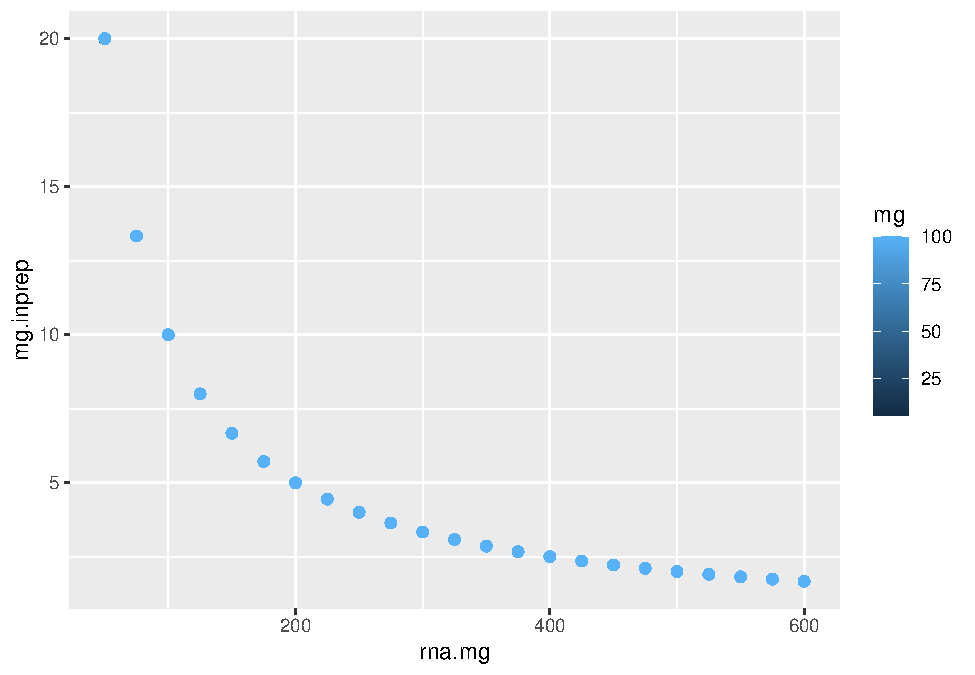
\includegraphics{thesis_files/figure-latex/unnamed-chunk-1-1.pdf}

\hypertarget{meta-analysis-of-within-session-training-volume}{%
\section{Meta-analysis of within-session training volume}\label{meta-analysis-of-within-session-training-volume}}

\hypertarget{literature-search-inclusion-criteria-and-coding-of-studies}{%
\subsection{Literature search, inclusion criteria and coding of studies}\label{literature-search-inclusion-criteria-and-coding-of-studies}}

A first set of studies were coded based previously published
meta-analyses (23,24). For more recent studies, PubMed, Google
Scholar and SportDiscuss searches were made with search terms being
``training volume,'' ``resistance training,'' ``strength training,'' ``set,''
``muscle strength,'' ``muscle hypertrophy'' used in different combinations.
Studies examining the effect of within-session training volume on muscle
strength and mass, with all other training variables kept constant
between study groups were considered for inclusion in the meta-analysis.
Studies were further assessed for inclusion based on criteria being; (i)
participants described as healthy without medications affecting muscle
metabolism, (ii) interventions lasting at least 6 weeks and (iii) RT
performed without additional stimuli (e.g.~blood flow restriction) at
intensities above 65\% of 1RM or 20RM.

All available outcome measures of muscle mass and strength gains in
response to RT were extracted from each study with exception of outcomes
reported both as summaries and individual measures (e.g.~muscle
thickness reported as individual muscles and summarized for the whole
muscle group). In such cases the summary was used as outcome. Weekly
training volume was calculated as product of weekly sessions, number of
sets and exercises for each muscle group assessed for muscle hypertrophy
or strength gains. An intervention average of weekly sessions was used
when the number of sessions per week differed over the course of the
intervention. An exercise was assumed to influence an outcome when it
targeted prime movers also assessed for strength or muscle hypertrophy
measures. Participant characteristics were coded based on sex (male,
female or mixed when a study failed to discern between male and
females), age (young, middle-aged, old or mixed), body-mass index (BMI,
calculated from average body mass and height when BMI values were not
available), training status (trained, \textgreater{} 1 session per week during the
last 6 months leading up to the intervention; untrained \textless{} 1 session).
Study groups were considered independent also in studies utilizing
within-participant models.

\hypertarget{calculations-of-effect-sizes-and-statistical-analysis}{%
\subsection{Calculations of effect sizes and statistical analysis}\label{calculations-of-effect-sizes-and-statistical-analysis}}

Group-wise effect sizes were calculated for each outcome measure based
on the within-group change score pre- to post-training divided by the
pre-training standard deviation (SD). Pre-training SD's were calculated
as a pooled SD within outcome and study. Variances of the effect size
were calculated using an average effect size across all outcomes within
muscle strength or mass, and correlations specific to each measurement
type (isokinetic-, isometric- or repetition maximum strength tests;
muscle thickness, magnetic resonance imaging, dual energy X‐ray
absorptiometry) estimated from previous studies.\\
A correction factor () was applied to both effect sizes and their
variances.

Mixed-effects meta-regression models were used to model the effect of
weekly number of sets on RT-induced muscle mass and strength gains.
Models were fitted in a Bayesian framework using the brms-package
(109).

\hypertarget{results-and-discussion}{%
\chapter{Results and Discussion}\label{results-and-discussion}}

\hypertarget{effects-of-different-training-volume-on-changes-in-muscle-size-and-function}{%
\section{Effects of different training volume on changes in muscle size and function}\label{effects-of-different-training-volume-on-changes-in-muscle-size-and-function}}

In Study I, the average increases (Table \ref{tab:csa-str-tab}) in muscle strength and mass in each volume condition corresponded to what could be expected based on previous studies
(110, 13).




\begin{table}

\caption{\label{tab:csa-str-tab}Training induced changes in muscle CSA and average strength in Study I}
\centering
\fontsize{7}{9}\selectfont
\begin{tabular}[t]{lllll}
\toprule
 & Sex & Volume condition & Mean (SD) & Reference\\
\midrule
 &  & LOW & 3.05 (3.61) & \\
\cmidrule{3-4}
 & \multirow{-2}{*}{\raggedright\arraybackslash Female} & MOD & 5.02 (4.04) & \\
\cmidrule{2-4}
 &  & LOW & 3.83 (3.50) & \\
\cmidrule{3-4}
\multirow{-4}{*}{\raggedright\arraybackslash CSA \%-change} & \multirow{-2}{*}{\raggedright\arraybackslash Male} & MOD & 5.10 (3.71) & \multirow{-4}{*}{\raggedright\arraybackslash }\\
\cmidrule{1-5}
 &  & LOW & 0.04 (0.05) & \\
\cmidrule{3-4}
 & \multirow{-2}{*}{\raggedright\arraybackslash Female} & MOD & 0.07 (0.05) & \\
\cmidrule{2-4}
 &  & LOW & 0.05 (0.05) & \\
\cmidrule{3-4}
\multirow{-4}{*}{\raggedright\arraybackslash CSA \%-change day} & \multirow{-2}{*}{\raggedright\arraybackslash Male} & MOD & 0.07 (0.05) & \multirow{-4}{*}{\raggedright\arraybackslash 0.11 [0.04-0.26]a}\\
\cmidrule{1-5}
 &  & LOW & 0.11 (0.13) & \\
\cmidrule{3-4}
 & \multirow{-2}{*}{\raggedright\arraybackslash Female} & MOD & 0.18 (0.15) & \multirow{-2}{*}{\raggedright\arraybackslash 0.08 (0.22)b}\\
\cmidrule{2-5}
 &  & LOW & 0.14 (0.12) & \\
\cmidrule{3-4}
\multirow{-4}{*}{\raggedright\arraybackslash CSA \%-change session} & \multirow{-2}{*}{\raggedright\arraybackslash Male} & MOD & 0.19 (0.13) & \multirow{-2}{*}{\raggedright\arraybackslash 0.14 (0.14)b}\\
\cmidrule{1-5}
 &  & LOW & 21.0 (9.8) & \\
\cmidrule{3-4}
 & \multirow{-2}{*}{\raggedright\arraybackslash Female} & MOD & 27.8 (14.4) & \\
\cmidrule{2-4}
 &  & LOW & 19.2 (12.4) & \\
\cmidrule{3-4}
\multirow{-4}{*}{\raggedright\arraybackslash Average strength \%-change} & \multirow{-2}{*}{\raggedright\arraybackslash Male} & MOD & 23.1 (12.0) & \multirow{-4}{*}{\raggedright\arraybackslash }\\
\cmidrule{1-5}
 &  & LOW & 0.77 (0.36) & \\
\cmidrule{3-4}
 & \multirow{-2}{*}{\raggedright\arraybackslash Female} & MOD & 1.00 (0.49) & \multirow{-2}{*}{\raggedright\arraybackslash 0.67 (0.35)b}\\
\cmidrule{2-5}
 &  & LOW & 0.72 (0.48) & \\
\cmidrule{3-4}
\multirow{-4}{*}{\raggedright\arraybackslash Average strength \%-session} & \multirow{-2}{*}{\raggedright\arraybackslash Male} & MOD & 0.87 (0.46) & \multirow{-2}{*}{\raggedright\arraybackslash 0.47 (0.22)b}\\
\bottomrule
\multicolumn{5}{l}{\textsuperscript{a} Estimates from Wernbom et al. (110)}\\
\multicolumn{5}{l}{\textsuperscript{b} Estimates from Ahtiainen et al. (ref:ahtiainen-citation}\\
\end{tabular}
\end{table}
Average within participant differences in responses between LOW and MOD were consistent across measures of muscle hypertrophy and strength gains (Figure \ref{fig:comb-fig-s1}). These differences were in agreement to what could be expected based on published meta-analyses
(79, 23, 22, 24).
Taken together, these observations confirmed the efficacy of training programs in general and a dose-response with regard to within-session exercise volume.

In Study II, training efficacy was assessed by comparing outcomes to a non-training control group. The training group displayed increases compared to the control group for both strength muscle thickness measures.
\begin{figure}

{\centering 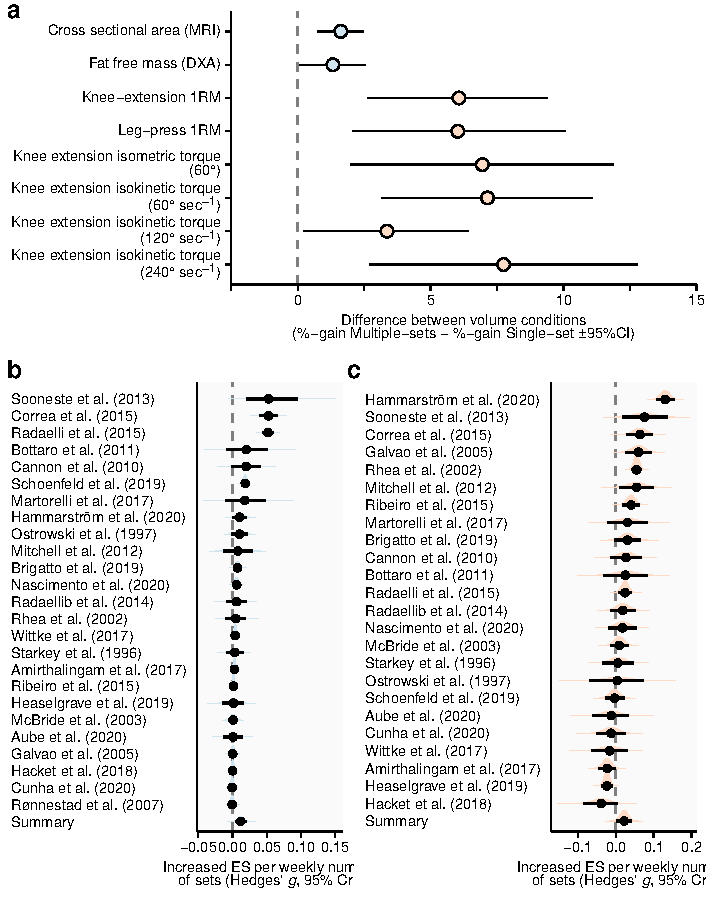
\includegraphics{thesis_files/figure-latex/comb-fig-s1-1} 

}

\caption[Differences in training induced changes to muscle mass and strength measures between volume conditions in Study I]{Differences in training induced relative changes in muscle mass and strength measures. Estimates are derived from ANCOVA models controling for baseline values and sex.}\label{fig:comb-fig-s1}
\end{figure}
\hypertarget{acute-effects-of-diffrent-training-volume-on-determinants-of-muscle-protein-synthesis}{%
\section{Acute effects of diffrent training volume on determinants of muscle protein synthesis}\label{acute-effects-of-diffrent-training-volume-on-determinants-of-muscle-protein-synthesis}}

\hypertarget{general-discussion}{%
\chapter{General Discussion}\label{general-discussion}}

\hypertarget{conclusion}{%
\chapter*{Conclusion}\label{conclusion}}
\addcontentsline{toc}{chapter}{Conclusion}

If we don't want Conclusion to have a chapter number next to it, we can add the \texttt{\{-\}} attribute.

\textbf{More info}

And here's some other random info: the first paragraph after a chapter title or section head \emph{shouldn't be} indented, because indents are to tell the reader that you're starting a new paragraph. Since that's obvious after a chapter or section title, proper typesetting doesn't add an indent there.

\backmatter

\hypertarget{references}{%
\chapter*{References}\label{references}}
\addcontentsline{toc}{chapter}{References}

\markboth{References}{References}

\noindent

\setlength{\parindent}{-0.20in}
\setlength{\leftskip}{0.20in}
\setlength{\parskip}{8pt}

\hypertarget{refs}{}
\begin{CSLReferences}{0}{0}
\leavevmode\hypertarget{ref-RN2512}{}%
\CSLLeftMargin{1. }
\CSLRightInline{Li R, Xia J, Zhang XI, Gathirua-Mwangi WG, Guo J, Li Y, et al. Associations of muscle mass and strength with all-cause mortality among US older adults. Medicine and science in sports and exercise {[}Internet{]}. 2018;50(3):458--67. }

\leavevmode\hypertarget{ref-RN2513}{}%
\CSLLeftMargin{2. }
\CSLRightInline{Fukasawa H, Kaneko M, Niwa H, Matsuyama T, Yasuda H, Kumagai H, et al. Lower thigh muscle mass is associated with all-cause and cardiovascular mortality in elderly hemodialysis patients. European Journal of Clinical Nutrition {[}Internet{]}. 2017;71(1):64--9. }

\leavevmode\hypertarget{ref-RN2514}{}%
\CSLLeftMargin{3. }
\CSLRightInline{Miyake H, Kanazawa I, Tanaka KI, Sugimoto T. Low skeletal muscle mass is associated with the risk of all-cause mortality in patients with type 2 diabetes mellitus. Ther Adv Endocrinol Metab {[}Internet{]}. 2019;10:2042018819842971. }

\leavevmode\hypertarget{ref-RN2376}{}%
\CSLLeftMargin{4. }
\CSLRightInline{Ruiz JR, Sui X, Lobelo F, Morrow Jr James R., Jackson AW, Sjöström M, et al. Association between muscular strength and mortality in men: Prospective cohort study. BMJ (Clinical research ed) {[}Internet{]}. 2008;337(7661):a439--9. }

\leavevmode\hypertarget{ref-RN2515}{}%
\CSLLeftMargin{5. }
\CSLRightInline{Szulc P, Munoz F, Marchand F, Chapurlat R, Delmas PD. Rapid loss of appendicular skeletal muscle mass is associated with higher all-cause mortality in older men: The prospective MINOS study. Am J Clin Nutr {[}Internet{]}. 2010;91(5):1227--36. }

\leavevmode\hypertarget{ref-RN2516}{}%
\CSLLeftMargin{6. }
\CSLRightInline{Abramowitz MK, Hall CB, Amodu A, Sharma D, Androga L, Hawkins M. Muscle mass, BMI, and mortality among adults in the united states: A population-based cohort study. PLoS One. 2018;13(4):e0194697. }

\leavevmode\hypertarget{ref-RN2517}{}%
\CSLLeftMargin{7. }
\CSLRightInline{Janssen I, Heymsfield SB, Ross R. Low relative skeletal muscle mass (sarcopenia) in older persons is associated with functional impairment and physical disability. J Am Geriatr Soc {[}Internet{]}. 2002;50(5):889--96. }

\leavevmode\hypertarget{ref-RN2532}{}%
\CSLLeftMargin{8. }
\CSLRightInline{Sousa AS, Guerra RS, Fonseca I, Pichel F, Ferreira S, Amaral TF. Financial impact of sarcopenia on hospitalization costs. Eur J Clin Nutr {[}Internet{]}. 2016;70(9):1046--51. }

\leavevmode\hypertarget{ref-RN2184}{}%
\CSLLeftMargin{9. }
\CSLRightInline{Pinedo-Villanueva R, Westbury LD, Syddall HE, Sanchez-Santos MT, Dennison EM, Robinson SM, et al. Health care costs associated with muscle weakness: A UK population-based estimate. Calcif Tissue Int {[}Internet{]}. 2019;104(2):137--44. }

\leavevmode\hypertarget{ref-RN763}{}%
\CSLLeftMargin{10. }
\CSLRightInline{Wolfe RR. The underappreciated role of muscle in health and disease. Am J Clin Nutr {[}Internet{]}. 2006;84(3):475--82. }

\leavevmode\hypertarget{ref-RN2526}{}%
\CSLLeftMargin{11. }
\CSLRightInline{Arden NK, Spector TD. Genetic influences on muscle strength, lean body mass, and bone mineral density: A twin study. Journal of Bone and Mineral Research {[}Internet{]}. 1997;12(12):2076--81. }

\leavevmode\hypertarget{ref-RN2527}{}%
\CSLLeftMargin{12. }
\CSLRightInline{Roth SM. Genetic aspects of skeletal muscle strength and mass with relevance to sarcopenia. BoneKEy reports {[}Internet{]}. 2012;1:58--8. }

\leavevmode\hypertarget{ref-RN1741}{}%
\CSLLeftMargin{13. }
\CSLRightInline{Ahtiainen JP, Walker S, Peltonen H, Holviala J, Sillanpaa E, Karavirta L, et al. Heterogeneity in resistance training-induced muscle strength and mass responses in men and women of different ages. Age (Dordr) {[}Internet{]}. 2016;38(1):10. }

\leavevmode\hypertarget{ref-RN2534}{}%
\CSLLeftMargin{14. }
\CSLRightInline{Grgic J, Garofolini A, Orazem J, Sabol F, Schoenfeld BJ, Pedisic Z. Effects of resistance training on muscle size and strength in very elderly adults: A systematic review and meta-analysis of randomized controlled trials. Sports Med {[}Internet{]}. 2020; }

\leavevmode\hypertarget{ref-RN2536}{}%
\CSLLeftMargin{15. }
\CSLRightInline{Faigenbaum AD, Myer GD. Resistance training among young athletes: Safety, efficacy and injury prevention effects. British Journal of Sports Medicine {[}Internet{]}. 2010;44(1):56. }

\leavevmode\hypertarget{ref-RN1}{}%
\CSLLeftMargin{16. }
\CSLRightInline{Ratamess N, Alvar BA, Evetoch TK, Housh TJ, Kibler B, Kraemer WJ, et al. American college of sports medicine position stand. Progression models in resistance training for healthy adults. Med Sci Sports Exerc {[}Internet{]}. 2009;41(3):687--708. }

\leavevmode\hypertarget{ref-RN798}{}%
\CSLLeftMargin{17. }
\CSLRightInline{Bird SP, Tarpenning KM, Marino FE. Designing resistance training programmes to enhance muscular fitness: A review of the acute programme variables. Sports Med {[}Internet{]}. 2005;35(10):841--51. }

\leavevmode\hypertarget{ref-RN2538}{}%
\CSLLeftMargin{18. }
\CSLRightInline{Feigenbaum MS, Pollock ML. Prescription of resistance training for health and disease. Med Sci Sports Exerc. 1999;31(1):38--45. }

\leavevmode\hypertarget{ref-RN791}{}%
\CSLLeftMargin{19. }
\CSLRightInline{Burd NA, Holwerda AM, Selby KC, West DW, Staples AW, Cain NE, et al. Resistance exercise volume affects myofibrillar protein synthesis and anabolic signalling molecule phosphorylation in young men. J Physiol {[}Internet{]}. 2010;588(Pt 16):3119--30. }

\leavevmode\hypertarget{ref-RN784}{}%
\CSLLeftMargin{20. }
\CSLRightInline{Terzis G, Spengos K, Mascher H, Georgiadis G, Manta P, Blomstrand E. The degree of p70 S6k and S6 phosphorylation in human skeletal muscle in response to resistance exercise depends on the training volume. Eur J Appl Physiol {[}Internet{]}. 2010;110(4):835--43. }

\leavevmode\hypertarget{ref-RN1837}{}%
\CSLLeftMargin{21. }
\CSLRightInline{Ahtiainen JP, Walker S, Silvennoinen M, Kyrolainen H, Nindl BC, Hakkinen K, et al. Exercise type and volume alter signaling pathways regulating skeletal muscle glucose uptake and protein synthesis. Eur J Appl Physiol. 2015;115(9):1835--45. }

\leavevmode\hypertarget{ref-RN793}{}%
\CSLLeftMargin{22. }
\CSLRightInline{Krieger JW. Single versus multiple sets of resistance exercise: A meta-regression. J Strength Cond Res {[}Internet{]}. 2009;23(6):1890--901. }

\leavevmode\hypertarget{ref-RN789}{}%
\CSLLeftMargin{23. }
\CSLRightInline{Krieger JW. Single vs. Multiple sets of resistance exercise for muscle hypertrophy: A meta-analysis. J Strength Cond Res {[}Internet{]}. 2010;24(4):1150--9. }

\leavevmode\hypertarget{ref-RN1767}{}%
\CSLLeftMargin{24. }
\CSLRightInline{Schoenfeld BJ, Ogborn D, Krieger JW. Dose-response relationship between weekly resistance training volume and increases in muscle mass: A systematic review and meta-analysis. J Sports Sci {[}Internet{]}. 2016;1--0. }

\leavevmode\hypertarget{ref-RN2063}{}%
\CSLLeftMargin{25. }
\CSLRightInline{Choi J, Lee M, Lee JK, Kang D, Choi JY. Correlates associated with participation in physical activity among adults: A systematic review of reviews and update. BMC Public Health {[}Internet{]}. 2017;17(1):356. }

\leavevmode\hypertarget{ref-RN794}{}%
\CSLLeftMargin{26. }
\CSLRightInline{Carpinelli RN, Otto RM. Strength training. Single versus multiple sets. Sports Med {[}Internet{]}. 1998;26(2):73--84. }

\leavevmode\hypertarget{ref-RN2547}{}%
\CSLLeftMargin{27. }
\CSLRightInline{Pickering C, Kiely J. Do non-responders to exercise exist---and if so, what should we do about them? Sports Medicine {[}Internet{]}. 2019;49(1):1--7. }

\leavevmode\hypertarget{ref-RN2640}{}%
\CSLLeftMargin{28. }
\CSLRightInline{Tipton CM. The history of "exercise is medicine" in ancient civilizations. Adv Physiol Educ {[}Internet{]}. 2014;38(2):109--17. }

\leavevmode\hypertarget{ref-RN2663}{}%
\CSLLeftMargin{29. }
\CSLRightInline{Pfister G. Cultural confrontations: German turnen, swedish gymnastics and english sport--european diversity in physical activities from a historical perspective. Culture, Sport, Society. 2003;6(1):61--91. }

\leavevmode\hypertarget{ref-RN2634}{}%
\CSLLeftMargin{30. }
\CSLRightInline{Nicoll EA. Principles of exercise therapy. British medical journal {[}Internet{]}. 1943;1(4302):747--50. }

\leavevmode\hypertarget{ref-RN2633}{}%
\CSLLeftMargin{31. }
\CSLRightInline{Delorme TL. RESTORATION OF MUSCLE POWER BY HEAVY-RESISTANCE EXERCISES. JBJS {[}Internet{]}. 1945;27(4). }

\leavevmode\hypertarget{ref-RN2639}{}%
\CSLLeftMargin{32. }
\CSLRightInline{Todd JS, Shurley JP, Todd TC. Thomas l. DeLorme and the science of progressive resistance exercise. J Strength Cond Res. 2012;26(11):2913--23. }

\leavevmode\hypertarget{ref-RN2641}{}%
\CSLLeftMargin{33. }
\CSLRightInline{Delorme TL, Watkins AL. Technics of progressive resistance exercise. Arch Phys Med Rehabil. 1948;29(5):263--73. }

\leavevmode\hypertarget{ref-RN2646}{}%
\CSLLeftMargin{34. }
\CSLRightInline{Delorme TL, West FE, Shriber WJ. INFLUENCE OF PROGRESSIVE-RESISTANCE EXERCISES ON KNEE FUNCTION FOLLOWING FEMORAL FRACTURES. JBJS {[}Internet{]}. 1950;32(4). }

\leavevmode\hypertarget{ref-RN2632}{}%
\CSLLeftMargin{35. }
\CSLRightInline{Houtz SJ, Parrish AM, Hellebrandt FA. The influence of heavy resistance exercise on strength. Physical Therapy {[}Internet{]}. 1946;26(6):299--304. }

\leavevmode\hypertarget{ref-RN2644}{}%
\CSLLeftMargin{36. }
\CSLRightInline{Chui E. The effect of systematic weight training on athletic power. Research Quarterly American Association for Health, Physical Education and Recreation {[}Internet{]}. 1950;21(3):188--94. }

\leavevmode\hypertarget{ref-RN2642}{}%
\CSLLeftMargin{37. }
\CSLRightInline{Capen EK. The effect of systematic weight training on power, strength, and endurance. Research Quarterly American Association for Health, Physical Education and Recreation {[}Internet{]}. 1950;21(2):83--93. }

\leavevmode\hypertarget{ref-RN2645}{}%
\CSLLeftMargin{38. }
\CSLRightInline{Hettinger T, Müller EA. Muskelleistung und muskeltraining. Arbeitsphysiologie {[}Internet{]}. 1953;15(2):111--26. }

\leavevmode\hypertarget{ref-RN1477}{}%
\CSLLeftMargin{39. }
\CSLRightInline{Capen EK. Study of four programs of heavy resistance exercises for development of muscular strength. Research Quarterly American Association for Health, Physical Education and Recreation {[}Internet{]}. 1956;27(2):132--42. }

\leavevmode\hypertarget{ref-RN1472}{}%
\CSLLeftMargin{40. }
\CSLRightInline{Galvao DA, Taaffe DR. Resistance exercise dosage in older adults: Single- versus multiset effects on physical performance and body composition. J Am Geriatr Soc {[}Internet{]}. 2005;53(12):2090--7. }

\leavevmode\hypertarget{ref-RN2659}{}%
\CSLLeftMargin{41. }
\CSLRightInline{Berger RA. COMPARISON OF THE EFFECT OF VARIOUS WEIGHT TRAINING LOADS ON STRENGTH. Res Q. 1965;36:141--6. }

\leavevmode\hypertarget{ref-RN2658}{}%
\CSLLeftMargin{42. }
\CSLRightInline{Berger RA, Hardage B. Effect of maximum loads for each of ten repetitions on strength improvement. Res Q. 1967;38(4):715--8. }

\leavevmode\hypertarget{ref-RN2656}{}%
\CSLLeftMargin{43. }
\CSLRightInline{O'Shea P. Effects of selected weight training programs on the development of strength and muscle hypertrophy. Res Q. 1966;37(1):95--102. }

\leavevmode\hypertarget{ref-RN2537}{}%
\CSLLeftMargin{44. }
\CSLRightInline{Fleck SJ, Kraemer WJ. Designing resistance training programs. Fourth edition. Champaign, IL: Human Kinetics; 2014. }

\leavevmode\hypertarget{ref-RN2655}{}%
\CSLLeftMargin{45. }
\CSLRightInline{American college of sports medicine position statement on the recommended quantity and quality of exercise for developing and maintaining fitness in healthy adults. Med Sci Sports. 1978;10(3):vii--x. }

\leavevmode\hypertarget{ref-RN2654}{}%
\CSLLeftMargin{46. }
\CSLRightInline{American college of sports medicine position stand. The recommended quantity and quality of exercise for developing and maintaining cardiorespiratory and muscular fitness in healthy adults. Med Sci Sports Exerc. 1990;22(2):265--74. }

\leavevmode\hypertarget{ref-RN2666}{}%
\CSLLeftMargin{47. }
\CSLRightInline{Manley AF. Physical activity and health: A report of the surgeon general. Diane Publishing; 1996. }

\leavevmode\hypertarget{ref-RN2667}{}%
\CSLLeftMargin{48. }
\CSLRightInline{Bull FC, Al-Ansari SS, Biddle S, Borodulin K, Buman MP, Cardon G, et al. World health organization 2020 guidelines on physical activity and sedentary behaviour. British journal of sports medicine {[}Internet{]}. 2020;54(24):1451--62. }

\leavevmode\hypertarget{ref-RN2696}{}%
\CSLLeftMargin{49. }
\CSLRightInline{Vol. 2021. }

\leavevmode\hypertarget{ref-RN2678}{}%
\CSLLeftMargin{50. }
\CSLRightInline{Sanford JA, Nogiec CD, Lindholm ME, Adkins JN, Amar D, Dasari S, et al. Molecular transducers of physical activity consortium (MoTrPAC): Mapping the dynamic responses to exercise. Cell {[}Internet{]}. 2020;181(7):1464--74. }

\leavevmode\hypertarget{ref-RN2677}{}%
\CSLLeftMargin{51. }
\CSLRightInline{Sparks LM. Exercise training response heterogeneity: Physiological and molecular insights. Diabetologia {[}Internet{]}. 2017;60(12):2329--36. }

\leavevmode\hypertarget{ref-RN764}{}%
\CSLLeftMargin{52. }
\CSLRightInline{Hubal MJ, Gordish-Dressman H, Thompson PD, Price TB, Hoffman EP, Angelopoulos TJ, et al. Variability in muscle size and strength gain after unilateral resistance training. Med Sci Sports Exerc {[}Internet{]}. 2005;37(6):964--72. }

\leavevmode\hypertarget{ref-RN1263}{}%
\CSLLeftMargin{53. }
\CSLRightInline{Pescatello LS, Devaney JM, Hubal MJ, Thompson PD, Hoffman EP. Highlights from the functional single nucleotide polymorphisms associated with human muscle size and strength or FAMuSS study. Biomed Res Int {[}Internet{]}. 2013;2013:643575. }

\leavevmode\hypertarget{ref-RN826}{}%
\CSLLeftMargin{54. }
\CSLRightInline{Thalacker-Mercer A, Stec M, Cui X, Cross J, Windham S, Bamman M. Cluster analysis reveals differential transcript profiles associated with resistance training-induced human skeletal muscle hypertrophy. Physiol Genomics {[}Internet{]}. 2013;45(12):499--507. }

\leavevmode\hypertarget{ref-RN2684}{}%
\CSLLeftMargin{55. }
\CSLRightInline{Stokes T, Timmons JA, Crossland H, Tripp TR, Murphy K, McGlory C, et al. Molecular transducers of human skeletal muscle remodeling under different loading states. Cell Rep. 2020;32(5):107980. }

\leavevmode\hypertarget{ref-RN2692}{}%
\CSLLeftMargin{56. }
\CSLRightInline{Crick F. Central dogma of molecular biology. Nature {[}Internet{]}. 1970;227(5258):561--3. }

\leavevmode\hypertarget{ref-RN2690}{}%
\CSLLeftMargin{57. }
\CSLRightInline{Seaborne RA, Sharples AP. The interplay between exercise metabolism, epigenetics, and skeletal muscle remodeling. Exerc Sport Sci Rev. 2020;48(4):188--200. }

\leavevmode\hypertarget{ref-RN2691}{}%
\CSLLeftMargin{58. }
\CSLRightInline{McGee SL, Hargreaves M. Epigenetics and exercise. Trends Endocrinol Metab. 2019;30(9):636--45. }

\leavevmode\hypertarget{ref-RN2683}{}%
\CSLLeftMargin{59. }
\CSLRightInline{Turner DC, Seaborne RA, Sharples AP. Comparative transcriptome and methylome analysis in human skeletal muscle anabolism, hypertrophy and epigenetic memory. Sci Rep {[}Internet{]}. 2019;9(1):4251. }

\leavevmode\hypertarget{ref-RN2012}{}%
\CSLLeftMargin{60. }
\CSLRightInline{Seaborne RA, Strauss J, Cocks M, Shepherd S, O'Brien TD, Someren KA van, et al. Human skeletal muscle possesses an epigenetic memory of hypertrophy. Sci Rep {[}Internet{]}. 2018;8(1):1898. }

\leavevmode\hypertarget{ref-RN2694}{}%
\CSLLeftMargin{61. }
\CSLRightInline{Yoshie T, Saito C, Kawano F. Early high-fat feeding improves histone modifications of skeletal muscle at middle-age in mice. Lab Anim Res {[}Internet{]}. 2020;36:25. }

\leavevmode\hypertarget{ref-RN2695}{}%
\CSLLeftMargin{62. }
\CSLRightInline{Godfrey KM, Costello PM, Lillycrop KA. Development, epigenetics and metabolic programming. Nestle Nutr Inst Workshop Ser {[}Internet{]}. 2016;85:71--80. }

\leavevmode\hypertarget{ref-RN758}{}%
\CSLLeftMargin{63. }
\CSLRightInline{Timmons JA. Variability in training-induced skeletal muscle adaptation. J Appl Physiol (1985) {[}Internet{]}. 2011;110(3):846--53. }

\leavevmode\hypertarget{ref-RN2681}{}%
\CSLLeftMargin{64. }
\CSLRightInline{Hautala AJ, Kiviniemi AM, Mäkikallio TH, Kinnunen H, Nissilä S, Huikuri HV, et al. Individual differences in the responses to endurance and resistance training. Eur J Appl Physiol {[}Internet{]}. 2006;96(5):535--42. }

\leavevmode\hypertarget{ref-RN346}{}%
\CSLLeftMargin{65. }
\CSLRightInline{Wernbom M, Augustsson J, Thomeé R. The influence of frequency, intensity, volume and mode of strength training on whole muscle cross-sectional area in humans. Sports Med {[}Internet{]}. 2007;37(3):225--64. }

\leavevmode\hypertarget{ref-RN752}{}%
\CSLLeftMargin{66. }
\CSLRightInline{Peterson MD, Sen A, Gordon PM. Influence of resistance exercise on lean body mass in aging adults: A meta-analysis. Med Sci Sports Exerc {[}Internet{]}. 2011;43(2):249--58. }

\leavevmode\hypertarget{ref-RN2669}{}%
\CSLLeftMargin{67. }
\CSLRightInline{Straight CR, Fedewa MV, Toth MJ, Miller MS. Improvements in skeletal muscle fiber size with resistance training are age-dependent in older adults: A systematic review and meta-analysis. Journal of Applied Physiology {[}Internet{]}. 2020;129(2):392--403. }

\leavevmode\hypertarget{ref-RN2629}{}%
\CSLLeftMargin{68. }
\CSLRightInline{Ikai M, Fukunaga T. A study on training effect on strength per unit cross-sectional area of muscle by means of ultrasonic measurement. Int Z Angew Physiol {[}Internet{]}. 1970;28(3):173--80. }

\leavevmode\hypertarget{ref-RN1710}{}%
\CSLLeftMargin{69. }
\CSLRightInline{Straight CR, Lindheimer JB, Brady AO, Dishman RK, Evans EM. Effects of resistance training on lower-extremity muscle power in middle-aged and older adults: A systematic review and meta-analysis of randomized controlled trials. Sports Medicine {[}Internet{]}. 2015;1--2. }

\leavevmode\hypertarget{ref-RN2608}{}%
\CSLLeftMargin{70. }
\CSLRightInline{Porter C, Reidy PT, Bhattarai N, Sidossis LS, Rasmussen BB. Resistance exercise training alters mitochondrial function in human skeletal muscle. Medicine and science in sports and exercise {[}Internet{]}. 2015;47(9):1922--31. }

\leavevmode\hypertarget{ref-RN2615}{}%
\CSLLeftMargin{71. }
\CSLRightInline{Ørtenblad N, Nielsen J, Boushel R, Söderlund K, Saltin B, Holmberg H-C. The muscle fiber profiles, mitochondrial content, and enzyme activities of the exceptionally well-trained arm and leg muscles of elite cross-country skiers. Frontiers in physiology {[}Internet{]}. 2018;9:1031--1. }

\leavevmode\hypertarget{ref-RN2575}{}%
\CSLLeftMargin{72. }
\CSLRightInline{Evans JW. Periodized resistance training for enhancing skeletal muscle hypertrophy and strength: A mini-review. Frontiers in physiology {[}Internet{]}. 2019;10:13--3. }

\leavevmode\hypertarget{ref-RN2572}{}%
\CSLLeftMargin{73. }
\CSLRightInline{Grgic J, Mikulic P, Podnar H, Pedisic Z. Effects of linear and daily undulating periodized resistance training programs on measures of muscle hypertrophy: A systematic review and meta-analysis. PeerJ {[}Internet{]}. 2017;5:e3695--5. }

\leavevmode\hypertarget{ref-RN2571}{}%
\CSLLeftMargin{74. }
\CSLRightInline{Schoenfeld BJ, Ogborn D, Krieger JW. Effects of resistance training frequency on measures of muscle hypertrophy: A systematic review and meta-analysis. Sports Med {[}Internet{]}. 2016;46(11):1689--97. }

\leavevmode\hypertarget{ref-RN2569}{}%
\CSLLeftMargin{75. }
\CSLRightInline{Schoenfeld BJ, Grgic J, Ogborn D, Krieger JW. Strength and hypertrophy adaptations between low- vs. High-load resistance training: A systematic review and meta-analysis. J Strength Cond Res. 2017;31(12):3508--23. }

\leavevmode\hypertarget{ref-RN1612}{}%
\CSLLeftMargin{76. }
\CSLRightInline{Schoenfeld BJ, Ratamess NA, Peterson MD, Contreras B, Sonmez GT, Alvar BA. Effects of different volume-equated resistance training loading strategies on muscular adaptations in well-trained men. J Strength Cond Res {[}Internet{]}. 2014;28(10):2909--18. }

\leavevmode\hypertarget{ref-RN2570}{}%
\CSLLeftMargin{77. }
\CSLRightInline{Grgic J, Schoenfeld BJ, Davies TB, Lazinica B, Krieger JW, Pedisic Z. Effect of resistance training frequency on gains in muscular strength: A systematic review and meta-analysis. Sports Med {[}Internet{]}. 2018;48(5):1207--20. }

\leavevmode\hypertarget{ref-RN2591}{}%
\CSLLeftMargin{78. }
\CSLRightInline{Nunes JP, Grgic J, Cunha PM, Ribeiro AS, Schoenfeld BJ, Salles BF de, et al. What influence does resistance exercise order have on muscular strength gains and muscle hypertrophy? A systematic review and meta-analysis. Eur J Sport Sci {[}Internet{]}. 2020;1--9. }

\leavevmode\hypertarget{ref-RN2492}{}%
\CSLLeftMargin{79. }
\CSLRightInline{Ralston GW, Kilgore L, Wyatt FB, Baker JS. The effect of weekly set volume on strength gain: A meta-analysis. Sports Med {[}Internet{]}. 2017;47(12):2585--601. }

\leavevmode\hypertarget{ref-RN2130}{}%
\CSLLeftMargin{80. }
\CSLRightInline{Baz-Valle E, Fontes-Villalba M, Santos-Concejero J. Total number of sets as a training volume quantification method for muscle hypertrophy: A systematic review. J Strength Cond Res. 2018; }

\leavevmode\hypertarget{ref-RN1476}{}%
\CSLLeftMargin{81. }
\CSLRightInline{Berger R. Effect of varied weight training programs on strength. Research Quarterly American Association for Health, Physical Education and Recreation {[}Internet{]}. 1962;33(2):168--81. }

\leavevmode\hypertarget{ref-RN2568}{}%
\CSLLeftMargin{82. }
\CSLRightInline{Junyoung H, Corinna NR, John DS, Sukho L. Low volume progressive single set of resistance training is as effective as high volume multiple sets of resistance protocol on muscle strength and power. International journal of applied sports sciences : IJASS. 2015;27(1):33--42. }

\leavevmode\hypertarget{ref-RN2201}{}%
\CSLLeftMargin{83. }
\CSLRightInline{Carpinelli RN. Science versus opinion. British journal of sports medicine {[}Internet{]}. 2004;38(2):240--2. }

\leavevmode\hypertarget{ref-RN2465}{}%
\CSLLeftMargin{84. }
\CSLRightInline{Ribeiro AS, Schoenfeld BJ, Pina FLC, Souza MF, Nascimento MA, Santos L dos, et al. Resistance training in older women: Comparison of single vs. Multiple sets on muscle strength and body composition. Isokinetics and Exercise Science. 2015;23:53--60. }

\leavevmode\hypertarget{ref-RN2464}{}%
\CSLLeftMargin{85. }
\CSLRightInline{Correa CS, Teixeira BC, Cobos RC, Macedo RC, Kruger RL, Carteri RB, et al. High-volume resistance training reduces postprandial lipaemia in postmenopausal women. J Sports Sci. 2015;33(18):1890--901. }

\leavevmode\hypertarget{ref-RN2463}{}%
\CSLLeftMargin{86. }
\CSLRightInline{Bottaro M, Veloso J, Wagner D, Gentil P. Resistance training for strength and muscle thickness: Effect of number of sets and muscle group trained. Science \& Sports {[}Internet{]}. 2011;26(5):259--64. }

\leavevmode\hypertarget{ref-RN1570}{}%
\CSLLeftMargin{87. }
\CSLRightInline{Radaelli R, Fleck SJ, Leite T, Leite RD, Pinto RS, Fernandes L, et al. Dose response of 1, 3 and 5 sets of resistance exercise on strength, local muscular endurance and hypertrophy. J Strength Cond Res {[}Internet{]}. 2014; }

\leavevmode\hypertarget{ref-RN1518}{}%
\CSLLeftMargin{88. }
\CSLRightInline{Radaelli R, Wilhelm EN, Botton CE, Rech A, Bottaro M, Brown LE, et al. Effects of single vs. Multiple-set short-term strength training in elderly women. Age (Dordr) {[}Internet{]}. 2014;36(6):9720. }

\leavevmode\hypertarget{ref-RN1474}{}%
\CSLLeftMargin{89. }
\CSLRightInline{McBride JM, Blaak JB, Triplett-McBride T. Effect of resistance exercise volume and complexity on EMG, strength, and regional body composition. Eur J Appl Physiol {[}Internet{]}. 2003;90(5-6):626--32. }

\leavevmode\hypertarget{ref-RN1456}{}%
\CSLLeftMargin{90. }
\CSLRightInline{Starkey DB, Pollock ML, Ishida Y, Welsch MA, Brechue WF, Graves JE, et al. Effect of resistance training volume on strength and muscle thickness. Med Sci Sports Exerc {[}Internet{]}. 1996;28(10):1311--20. }

\leavevmode\hypertarget{ref-RN1454}{}%
\CSLLeftMargin{91. }
\CSLRightInline{Ostrowski KJ, Wilson GJ, Weatherby R, Murphy PW, Lyttle AD. The effect of weight training volume on hormonal output and muscular size and function. Journal of Strength and Conditioning Research {[}Internet{]}. 1997;11(3):148--54. }

\leavevmode\hypertarget{ref-RN1384}{}%
\CSLLeftMargin{92. }
\CSLRightInline{Rhea MR, Alvar BA, Ball SD, Burkett LN. Three sets of weight training superior to 1 set with equal intensity for eliciting strength. J Strength Cond Res {[}Internet{]}. 2002;16(4):525--9. }

\leavevmode\hypertarget{ref-RN1382}{}%
\CSLLeftMargin{93. }
\CSLRightInline{Cannon J, Marino FE. Early-phase neuromuscular adaptations to high- and low-volume resistance training in untrained young and older women. J Sports Sci {[}Internet{]}. 2010;28(14):1505--14. }

\leavevmode\hypertarget{ref-RN776}{}%
\CSLLeftMargin{94. }
\CSLRightInline{Ronnestad BR, Egeland W, Kvamme NH, Refsnes PE, Kadi F, Raastad T. Dissimilar effects of one- and three-set strength training on strength and muscle mass gains in upper and lower body in untrained subjects. J Strength Cond Res {[}Internet{]}. 2007;21(1):157--63. }

\leavevmode\hypertarget{ref-RN834}{}%
\CSLLeftMargin{95. }
\CSLRightInline{Mitchell CJ, Churchward-Venne TA, West DW, Burd NA, Breen L, Baker SK, et al. Resistance exercise load does not determine training-mediated hypertrophic gains in young men. J Appl Physiol (1985) {[}Internet{]}. 2012;113(1):71--7. }

\leavevmode\hypertarget{ref-RN1607}{}%
\CSLLeftMargin{96. }
\CSLRightInline{Sooneste H, Tanimoto M, Kakigi R, Saga N, Katamoto S. Effects of training volume on strength and hypertrophy in young men. J Strength Cond Res {[}Internet{]}. 2013;27(1):8--13. }

\leavevmode\hypertarget{ref-RN2563}{}%
\CSLLeftMargin{97. }
\CSLRightInline{Lin CH, Platt MD, Ficarro SB, Hoofnagle MH, Shabanowitz J, Comai L, et al. Mass spectrometric identification of phosphorylation sites of rRNA transcription factor upstream binding factor. Am J Physiol Cell Physiol {[}Internet{]}. 2007;292(5):C1617--24. }

\leavevmode\hypertarget{ref-RN2602}{}%
\CSLLeftMargin{98. }
\CSLRightInline{Voit R, Hoffmann M, Grummt I. Phosphorylation by G1-specific cdk-cyclin complexes activates the nucleolar transcription factor UBF. Embo j {[}Internet{]}. 1999;18(7):1891--9. }

\leavevmode\hypertarget{ref-RN2604}{}%
\CSLLeftMargin{99. }
\CSLRightInline{Stefanovsky VY, Pelletier G, Hannan R, Gagnon-Kugler T, Rothblum LI, Moss T. An immediate response of ribosomal transcription to growth factor stimulation in mammals is mediated by ERK phosphorylation of UBF. Molecular Cell {[}Internet{]}. 2001;8(5):1063--73. }

\leavevmode\hypertarget{ref-RN2618}{}%
\CSLLeftMargin{100. }
\CSLRightInline{Newlands S, Levitt LK, Robinson CS, Karpf AB, Hodgson VR, Wade RP, et al. Transcription occurs in pulses in muscle fibers. Genes \& development {[}Internet{]}. 1998;12(17):2748--58. }

\leavevmode\hypertarget{ref-RN2616}{}%
\CSLLeftMargin{101. }
\CSLRightInline{Kirby TJ, Patel RM, McClintock TS, Dupont-Versteegden EE, Peterson CA, McCarthy JJ. Myonuclear transcription is responsive to mechanical load and DNA content but uncoupled from cell size during hypertrophy. Molecular biology of the cell {[}Internet{]}. 2016;27(5):788--98. }

\leavevmode\hypertarget{ref-RN2548}{}%
\CSLLeftMargin{102. }
\CSLRightInline{World medical association declaration of helsinki: Ethical principles for medical research involving human subjects. Jama {[}Internet{]}. 2013;310(20):2191--4. }

\leavevmode\hypertarget{ref-RN824}{}%
\CSLLeftMargin{103. }
\CSLRightInline{Hayot M, Michaud A, Koechlin C, Caron MA, Leblanc P, Prefaut C, et al. Skeletal muscle microbiopsy: A validation study of a minimally invasive technique. Eur Respir J {[}Internet{]}. 2005;25(3):431--40. }

\leavevmode\hypertarget{ref-RN2549}{}%
\CSLLeftMargin{104. }
\CSLRightInline{Ekblom B. The muscle biopsy technique. Historical and methodological considerations. Scand J Med Sci Sports {[}Internet{]}. 2017;27(5):458--61. }

\leavevmode\hypertarget{ref-RN2553}{}%
\CSLLeftMargin{105. }
\CSLRightInline{Bonafiglia JT, Islam H, Preobrazenski N, Drouin P, Ma A, Gerhart A, et al. A comparison of pain responses, hemodynamic reactivity and fibre type composition between bergström and microbiopsy skeletal muscle biopsies. Current Research in Physiology {[}Internet{]}. 2020;3:1--0. }

\leavevmode\hypertarget{ref-RN2552}{}%
\CSLLeftMargin{106. }
\CSLRightInline{Hughes MC, Ramos SV, Turnbull PC, Nejatbakhsh A, Baechler BL, Tahmasebi H, et al. Mitochondrial bioenergetics and fiber type assessments in microbiopsy vs. Bergstrom percutaneous sampling of human skeletal muscle. Frontiers in Physiology {[}Internet{]}. 2015;6(360). }

\leavevmode\hypertarget{ref-RN874}{}%
\CSLLeftMargin{107. }
\CSLRightInline{Blomstrand E, Ekblom B. The needle biopsy technique for fibre type determination in human skeletal muscle--a methodological study. Acta Physiol Scand {[}Internet{]}. 1982;116(4):437--42. }

\leavevmode\hypertarget{ref-RN2672}{}%
\CSLLeftMargin{108. }
\CSLRightInline{Chomczynski P, Sacchi N. Single-step method of RNA isolation by acid guanidinium thiocyanate-phenol-chloroform extraction. Analytical Biochemistry {[}Internet{]}. 1987;162(1):156--9. }

\leavevmode\hypertarget{ref-RN2562}{}%
\CSLLeftMargin{109. }
\CSLRightInline{Bürkner P-C. Brms: An r package for bayesian multilevel models using stan. 2017 {[}Internet{]}. 2017;80(1):28. }

\leavevmode\hypertarget{ref-RN2007}{}%
\CSLLeftMargin{110. }
\CSLRightInline{Bland M. An introduction to medical statistics. Fourth edition. Oxford ; Oxford University Press; 2015. (Oxford medical publications). }

\end{CSLReferences}

% Index?

\end{document}
